\section{Bezier Curves}

I would highly recommend watching \href{https://www.youtube.com/watch?v=jvPPXbo87ds&t=2384s}{this YouTube video} for a detailed explanation of the topic. \medskip

One way of modelling a geometric object are Bezier curves. Bezier curves are defines as:
$$x(t) = b_0 B_0^n(t) + ... + b_n B_n^n(t)$$

Where $B_i^n(t)$ is a Bernstein polynomial of degree $n$:
$$B_i^n(t) = {n \choose i} t^i (1-t)^{n-1} \qquad i < 0, i > n: B_i^n(t) = 0$$

Bernstein polynomials are positive definite and provide global support. Bezier curves can be thought consecutive interpolation. 
\begin{center}
	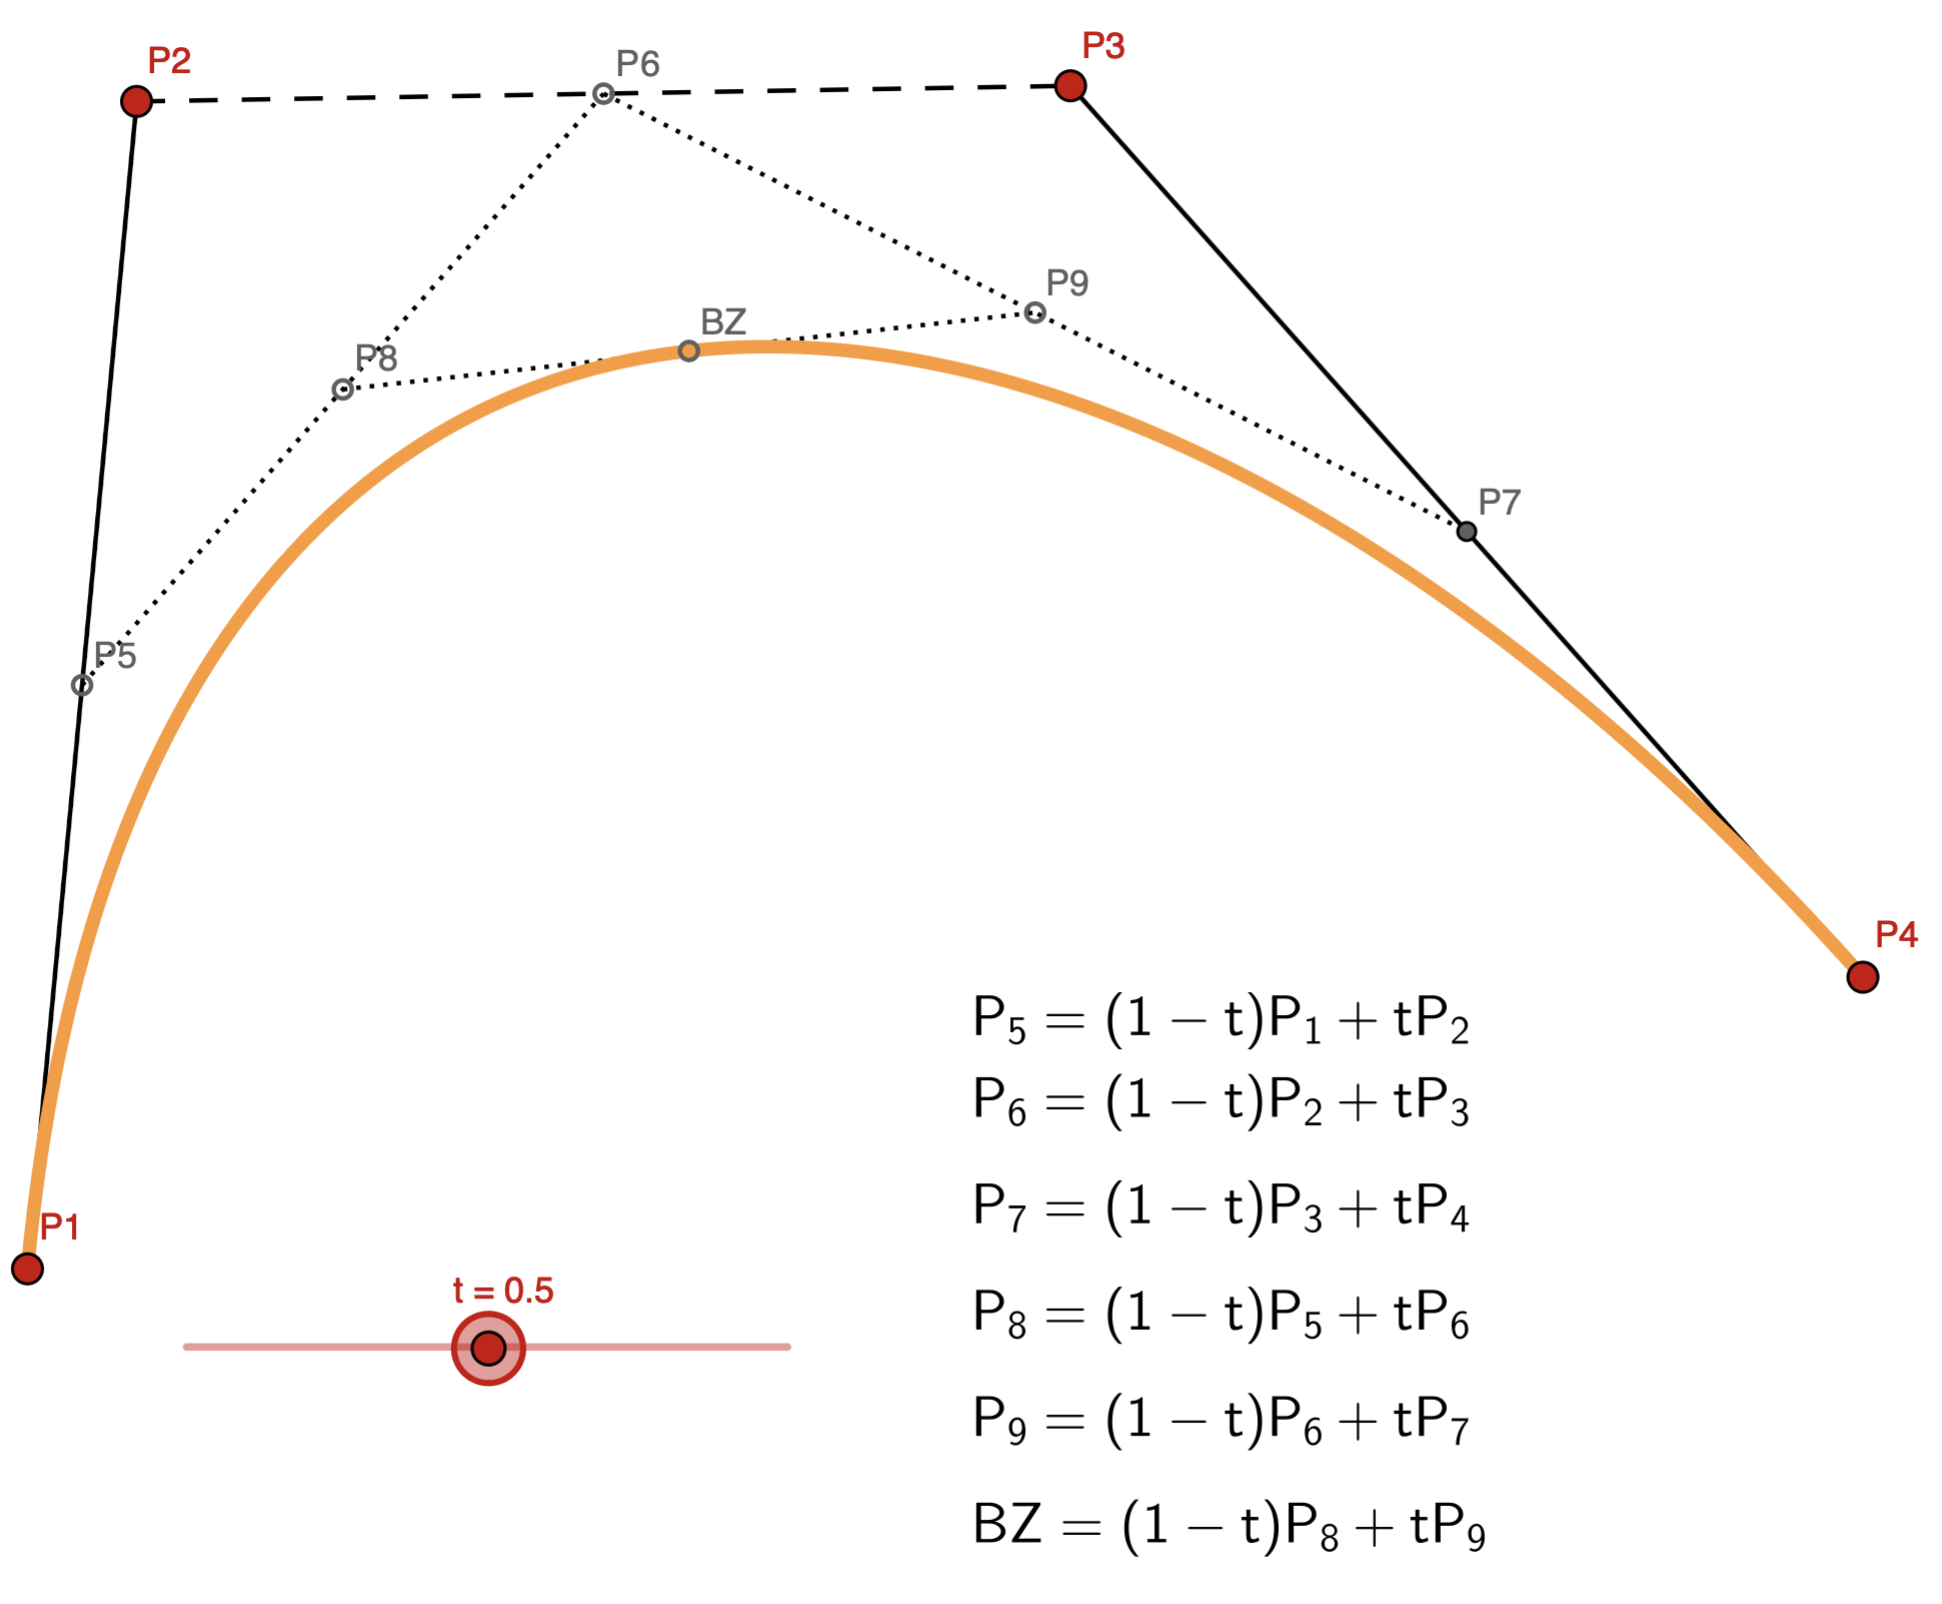
\includegraphics[width=\linewidth]{bezier.png}
\end{center}

This leads to deCasteljau's algorithm, $\mathcal O (n^2)$. One of the downsides when combining Bezier curves is that the are only $C_0$ smooth.
